\section{Tallgrass Prairie National Preserve}\label{app:TAPR}

\subsection{Current Grassland Management Goals and Programs}

\subsubsection{Grassland Management Goals}

\paragraph{Maintain tallgrass prairie remnant} 
Tallgrass Prairie National Preserve (TAPR) is unique in that they were explicitly created to protect the prairie and the cultural impact of the tallgrass prairie in the Kansas Flint Hills. 
This allows all management focus to center on maintaining a native prairie and all of the processes and resources that depend on that goal. 
Relics of legacy land use have created some areas of non-native prairie.
Restoration is ongoing to restore bottomlands to native species.

\paragraph{Wildlife habitat} 
TAPR is not focused on single resource pertaining to wildlife. 
Other units in this study focus on the vigor of individual wildlife species.
The wording of management documents at TAPR is vastly different. 
Rather than managing for wildlife species, their management documents focus on the prairie and the habitat that it can provide for a multitude of species.
Similarly, although the Topeka Shiner is a key threatened species in the unit, TAPR is focused on improving aquatic habitat via altered cattle grazing. 
This is a systems focus that will benefit the resilience of the grassland.

\paragraph{Upland stream maintenance} 
The Topeka Shiner is an endangered species present in prairie streams flowing through TAPR. 
Partnerships with state agencies and academic researchers have focused on the status of this fish and the habitat it depends on. 
Due to its importance as an endangered species, the unit is looking into how to best manage for the stream habitat in upland areas of the unit.

\subsubsection{Grassland Management Programs}

\paragraph{Mechanical removal of woody species} 
TAPR is extremely susceptible to woody encroachment. 
As such, they have an extensive management program to remove these invasive species. 
Constant efforts make headway, but unit staff expressed the need for more focused management on herbaceous invasive species rather than a constant battle against woody encroachment.

\paragraph{Bison management} 
Bison were reintroduced to TAPR in 2009. 
They are managed as a satellite herd of the Wind Cave NP population. 
More animals may be introduced in the future to maintain the genetics of this population as they currently do not maintain enough animals to continue as a viable herd. 
Bison are stocked year round and grazing is coupled with fire to impose disturbance on the landscape at TAPR.

\paragraph{Cattle management} 
The Flint Hills have a ranching history that is part of the cultural narrative of TAPR. 
Establishment of the unit required that cattle continue to graze on some lands within the unit. 
A lessee is allotted a certain amount of AUMs each season and the park manages cattle under different management systems such as early intensive grazing.
There is also fire coupled with livestock grazing.
Recently, stocking rates have been lower and monitoring shows vegetation has slightly declined in quality \citep{leis2018}.

\begin{table}[h]
	\centering
\caption[TAPR management documents]
	{Management documents for TAPR published from 2008-2018}
\label{tab:TAPRmandocs}
\begin{tabular}{lc}
		\toprule
		Title & Year\tabularnewline
		\midrule
Bison Management Plan & 2009 \tabularnewline
Fire Management Plan & 2016 \tabularnewline
TAPR General Agreement & 2016 \tabularnewline
Foundation Document & 2017 \tabularnewline
\bottomrule
\end{tabular}
\end{table}

\subsection{Management Plans and Data Available}

\subsubsection{Management Plans}

TAPR is a newer NPS unit established, in its current form, in 2005.
There are fewer published plans because of this. 
At this unit, more so than others, interviews revealed that management decisions are made adaptively either seasonally or annually. 
This is communicated as both positive and negative. 
Positive, as they are able to make changes quickly to address management issues. 
Negative, because there aren't clear goals they are working towards other than the broad goal of a healthy native ecosystem. 
The partnership between NPS and TNC makes it especially important to have clear goals that both parties agree on for management. 
Published management plans are listed in Table~\ref{tab:TAPRmandocs}.

\subsubsection{Data Available}

Water, wildlife and vegetation are of equal study at TAPR. 
The unit is less dependent on I\&M data as outside agencies and outside researchers contribute a significant amount of research to the unit. 
The status of resources is highly documented which means expansion of the disturbance regime would be plausible. 
The continuation of management decision making may be more challenging as there are not consistent programs in the currently available data (Table~\ref{tab:TAPRdata}).

%\storeareas\normalsetting
\KOMAoption{paper}{landscape}
\areaset{1.5\textwidth}{.6\textheight}
\recalctypearea
\pagestyle{plain}
\setlength\LTcapwidth{1.5\textwidth} 
\setlength\LTleft{0pt}           
\begin{longtable}[l]{@{}p{5cm}p{2cm}p{3cm}p{4cm}p{3cm}p{4cm}p{3cm}@{}}
	\caption[TAPR data]
	{Selected data collected in TAPR, 2008-2018.} 
	\label{tab:TAPRdata} \\
	\toprule
	Data title & Data type & Spatial extent & Frequency & Duration & Collecting agency & Format located \tabularnewline
	\midrule
	\endfirsthead 
	\caption* {\textbf{Table \ref{tab:TAPRdata}}, \emph{continued.}} \\
\toprule
	Data title & Data type & Spatial extent & Frequency & Duration & Collecting agency & Format located \tabularnewline
\midrule
\endhead
Night Skies and Photic Environment Resource Summary & Air & unit wide & compiled once & 2013 & NPS & on network\tabularnewline
Soil Survey & Geology & unit wide & once & 2010 & NPS/ USDA/ NRCS & on network\tabularnewline
Lithology and Paleontology of the Stratigraphic Units Cropping out TAPR & Geology & unit wide & written 2008 & park historical report & Kansas Geological Survey & on network\tabularnewline
Fixed Point Repeat Photography & Vegetation & preserve wide and outside preserve for comparison & once per year & 1997- 2015 & NPS/ TNC & on network\tabularnewline
Vegetation Classification and Mapping of TAPR & Vegetation & Preserve wide & Data collected once & July 2008 & Kansas Natural Heritage Survey & Online search\tabularnewline
Grazing Stocking Database & Vegetation & pastures with stocked grazers & updated annually & 1995-current & NPS/ TNC & on network\tabularnewline
Restoration Transect Data & Vegetation & different fields with restoration ongoing & summer & 2013 & NPS & on network\tabularnewline
TAPR Post Burn Summaries & Vegetation & fire patch varies each year & post fire & once after each annual burn & NPS/Heartland Network & IRMA\tabularnewline
Evaluating Long- term trends in vegetation and management intensity & Vegetation & unit wide & vegetation data collected once every four years by Heartland network & 1995-2014 & NPS/ Heartland Network &
IRMA\tabularnewline
Assessing Fluvial Geomorphology Conditions of Upland Prairie Stream Reaches on the Tallgrass Prairie National Preserve & Water & unit wide & once per year & 2006-2016 & Kansas State University/ The Watershed Institute & on network\tabularnewline
Palmer Creek Water Assessment & Water & Palmer Creek & one trip & 2015 & KDWP & on network\tabularnewline
Palmer Creek Fluvial Geomorphology & Water & Palmer Creek & once in the season & 2009 & The Watershed Institute & on network\tabularnewline
Fox Creek Hydrology & Water & Fox Creek & sensors collecting frequently throughout the years & 2009-2013 & NPS & on network\tabularnewline
Fish Assemblage Survey & Wildlife & all ponds on the preserve through seining & once per pond & April- June 2014 & Emporia State University & on network\tabularnewline
Bat Surveys & Wildlife & unit wide & one season & 17 nights from May-June 2017 & NPS/ TNC & on network\tabularnewline
Butterfly Count Site Totals & Wildlife & unit wide & each season & 2009-2016 & NPS/ other investigators & on network\tabularnewline
Wildlife Fire Effects & Wildlife & unit wide & yearly effects collected & 2010 & Missouri State University & IRMA\tabularnewline
Fishes in Lower Fox Creek & Wildlife & unit wide & May- August 2014 & 2014 & Emporia State University & on network\tabularnewline
Lek Data & Wildlife & unit wide & once per year & 2008-2011 & NRCS & on network\tabularnewline
Butterfly Inventory and Effects of Fire and Grazing & Wildlife & 6 transects per management unit & once & 7-10 day period each month from May -Sept & Emporia State University & on network\tabularnewline
Impacts of Alternative Grassland Management Regimes on the Population Ecology of Grassland Birds & Wildlife & land across the Flint Hills region & 463 surveys 156 different 300m line transects & Feb 2011- Feb 2014 & KSU, MSU, Benedictine College & on network\tabularnewline
Fishes of TAPR & Wildlife & lower Fox Creek & once in 2014 & 30 May to 12 August 2014 but compiling with other previously collected data 2018 & NPS/ Emporia State University & on network\tabularnewline
Semiaquatic turtles of TAPR & Wildlife & Fox Creek & 21 dates & 14 June - 18 September 2014 & Emporia State University & on network\tabularnewline
Kansas Winter Bird Count & Wildlife & unit wide & once each winter & have data from 2016-2018 & NPS & on network\tabularnewline
Monitoring Summary for TAPR of Bird Communities & Wildlife & 58 points unit wide & yearly effects collected & May 14- June 12 & NPS & on network\tabularnewline
USFWS FH Bird Survey & Wildlife & 51 sampling routes & yearly effects collected & March- May 2013 & TNC/ USFWS/ volunteers & on network\tabularnewline
\bottomrule
\end{longtable}
\clearpage
\normalsetting
\pagestyle{fancy} 

\subsection{Disturbance Regime }
\label{ref:TAPR_PBG}
\subsubsection{Grazing }

Cattle and bison are managed at TAPR in conjunction with ecological objectives. 
Bison were reintroduced to TAPR in 2009 with animals from Wind Cave NP and are managed in separate pastures\textemdash  cattle only graze for 90 days in an early intensive stocking system. 
Cattle stocking rates are assigned each year by TNC staff at TAPR based off of the previous year's conditions. 
Bison are also rounded up annually to determine herd size and health.
 A coupled disturbance regime is used at TAPR, which entails moving grazers through the landscape using burning as an attractant. 
This is beneficial to protect sensitive streams from grazer impact. 
Grazing is also somewhat unnaturally managed so that tall grass is present for visitor experience. 
Fire can also be used to move grazers away from certain visitor heavy areas.

\subsubsection{Fire }

TAPR monitoring follows national fire effects guidelines as per the fire effects guidebook. 
The plant community monitoring protocol states that, ``resource limitations have
resulted in sampling designs oriented toward short-term, burn unit-specific information to determine whether the objectives of a specific prescribed fire or mechanical treatment project have been met.'' 
There is heterogeneity present in a patch burn grazing system at TAPR (Fig.~\ref{fig:TAPRfiremosaic}). 
Prescribed fires have been conducted in varying seasons in recent years. 
This is beneficial to the ecosystem increasing pyro-diversity. 
Variety in fire behavior and fire season mimics the natural disturbance regime.

\begin{figure}
	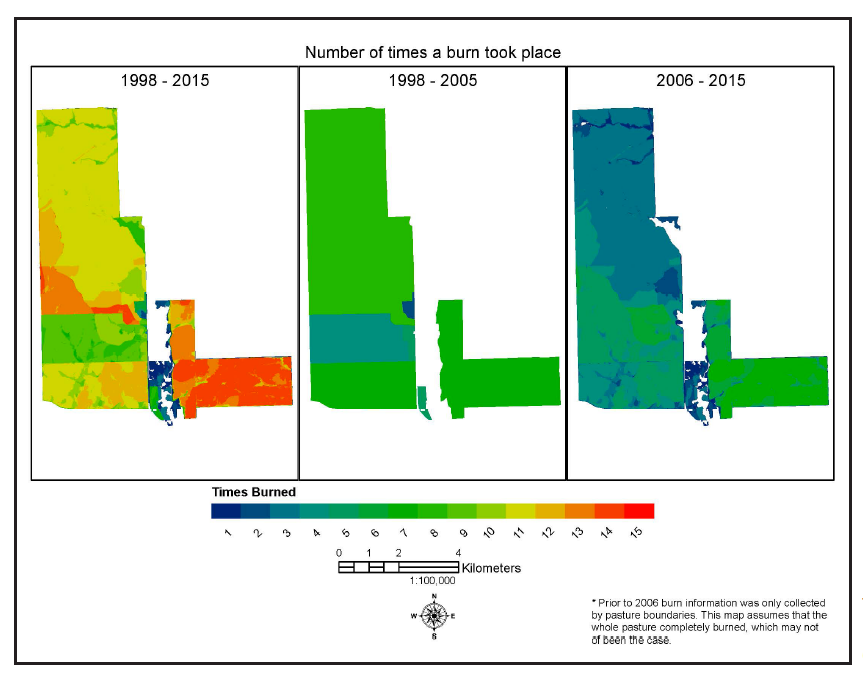
\includegraphics[width=1\textwidth]{TAPR_Fire_mosaic}
	\caption[TAPR fire mosaic]
	{Mosaic created through patch burn grazing at TAPR \citep{leis2018}. }
	\label{fig:TAPRfiremosaic}
\end{figure}

\subsection{Data gaps and suggested research}

\subsubsection{Data Gaps}

To implement further heterogeneity through a coupled disturbance regime, there are several areas where TAPR could collect further data. 
Formal overall status of resources is lacking. 
The four other parks in this study have a complete Natural Resource Condition Assessment (NRCA) detailing the resources protected. 
TAPR does not have this document. 
An overall assessment of resources at the unit would aid in the establishment of a standard disturbance regime. 
Available data is consistently a one-time study or collected over several years and then halted due to staff or budget constraints. 
Unit staff stressed the need for consistent annual data to make decisions off of. 
TAPR is unique in that the Heartland I\&M network only surveys the unit once every four
years rather than annually which is typical for other NPS units in this study.

More consistent data is also needed on invasive species management and seasonal wildlife populations. 
Staff mentioned adaptive management, but not having ``hard'' data to inform these annual decisions. 
TAPR has a coupled disturbance regime occurring on several areas of the unit.
Annual data on grazer forage demand and productivity are needed to optimize the fire-grazing interaction as a disturbance regime. 
Unit staff also expressed desires to better manage for prairie streams and the threatened Topeka Shiner. 
As such, there is data missing on grazer impact on water resources as well as erosion rates in high use areas.

\subsubsection{Suggested Research}

The disturbance regime at TAPR has a high level of established heterogeneity. 
Patch-burn grazing has created diversity on the landscape that benefits wildlife species. 
Annual management is required in an ongoing disturbance regime. 
Disturbances cannot be applied once in a while as a tool but must be a continuous process. 
Invasive species management is a major issue at TAPR. 
This includes both herbaceous and woody species. 
Goals need to be established for management of these species. 
Fire and grazing might have impacts, but goals need to be established to prescribe an effective disturbance regime.

\begin{itemize}
\item   The effects of grazing on erosion and water resources/aquatic species
\item   Range utilization collected each year
\end{itemize}

\subsection{Management Recommendations} 

\subsubsection{Expand coupled disturbance regime}

Expanding the coupled disturbance regime at TAPR will increase the resilience of the tallgrass prairie. 
Expanding the disturbance process can also help manage more of the landscape affected by invasive species. 
\emph{Sericea lespedeza} is a critical concern at TAPR. 
Late spring burning or fall burning are known to affect this species, but further research in the context of the landscape at TAPR would be beneficial to understand the best course of action.

\subsubsection{Target woody encroachment }
 
Mechanical treatment of woody invasives is time-intensive.
Strapped budgets and staff at TAPR could be used in many other ways if woody species were targeted via a natural disturbance regime. 
Preliminary data suggest fall burns and more intense burns can reduce woody species in tallgrass prairie \citep{weir2017}. 
TAPR has begun to burn in other seasons, but researching the impacts and communicating these to the public could make the use of fall prescribed fires more acceptable to surrounding landowners.

